\documentclass[a4paper]{article}
\usepackage{fullpage} % Package to use full page
\usepackage{parskip} % Package to tweak paragraph skipping
\usepackage{tikz} % Package for drawing
\usepackage{amsmath}
\usepackage{hyperref}
\usepackage{amssymb}
\usepackage{listings}
\usepackage{enumerate}
%%%%%%
\usepackage{color}

\definecolor{mygreen}{rgb}{0,0.6,0}
\definecolor{mygray}{rgb}{0.5,0.5,0.5}
\definecolor{mymauve}{rgb}{0.58,0,0.82}

\lstset{ %
  backgroundcolor=\color{white},   % choose the background color; you must add \usepackage{color} or \usepackage{xcolor}; should come as last argument
  basicstyle=\footnotesize,        % the size of the fonts that are used for the code
  breakatwhitespace=false,         % sets if automatic breaks should only happen at whitespace
  breaklines=true,                 % sets automatic line breaking
  captionpos=b,                    % sets the caption-position to bottom
  commentstyle=\color{mygreen},    % comment style
  deletekeywords={...},            % if you want to delete keywords from the given language
  escapeinside={\%*}{*)},          % if you want to add LaTeX within your code
  extendedchars=true,              % lets you use non-ASCII characters; for 8-bits encodings only, does not work with UTF-8
  frame=single,                    % adds a frame around the code
  keepspaces=true,                 % keeps spaces in text, useful for keeping indentation of code (possibly needs columns=flexible)
  keywordstyle=\color{blue},       % keyword style
  language=Octave,                 % the language of the code
  morekeywords={*,...},           % if you want to add more keywords to the set
  numbers=left,                    % where to put the line-numbers; possible values are (none, left, right)
  numbersep=5pt,                   % how far the line-numbers are from the code
  numberstyle=\tiny\color{mygray}, % the style that is used for the line-numbers
  rulecolor=\color{black},         % if not set, the frame-color may be changed on line-breaks within not-black text (e.g. comments (green here))
  showspaces=false,                % show spaces everywhere adding particular underscores; it overrides 'showstringspaces'
  showstringspaces=false,          % underline spaces within strings only
  showtabs=false,                  % show tabs within strings adding particular underscores
  stepnumber=2,                    % the step between two line-numbers. If it's 1, each line will be numbered
  stringstyle=\color{mymauve},     % string literal style
  tabsize=2,                       % sets default tabsize to 2 spaces
  title=\lstname                   % show the filename of files included with \lstinputlisting; also try caption instead of title
}

%%%%%%
\title{Assignment 1 for \#70240413 \\ "Statistical Machine Learning" }
\author{Kui XU, 2016311209}
\date{2017/03/23}

\begin{document}

\maketitle

\section{Mathematics Basics}

Choose one problem from the 1.1 and 1.2. A bonus would be given if you finished the both.

\subsection{Calculus}
The gamma function is defined by (assuming x $>$ 0)

\begin{equation}
\Gamma (x) = \int^{\infty}_{0}{u^{x-1}e^{-u}du.}
\end{equation}

\begin{enumerate}
\item[(1)] Prove that $\Gamma (x + 1) =x \Gamma (x)$.
\item[(2)] Also show that 
            \begin{equation}
            \int^{1}_{0}{u^{a-1}{(1-u)}^{b-1}du=\frac{\Gamma(a)\Gamma(b)}{\Gamma (a+b)}.}
            \end{equation}
\end{enumerate}


\textbf{Solution:} For Question (1), we can prove it by Using integration by parts, the steps are as follows:
\begin{equation}
    \begin{aligned}
        \Gamma(x+1) &= \int_0^\infty u^{x} e^{-u}\,du \\
                    &= \left[-u^x e^{-u}\right]_0^\infty + \int_0^\infty x u^{x-1} e^{-u}\, du \\
                    &= \lim_{u\to \infty}(-u^x e^{-u}) - (0 e^{-0}) + x\int_0^\infty u^{x-1} e^{-u}\, du \\
                    &= x\int_0^\infty u^{x-1} e^{-u}\, du\\
                    &= x\Gamma(x)
    \end{aligned}
\end{equation}
As we know, when $u\to \infty$, $-u^x e^{-u}\to 0$, so the equation is proved.\\



\textbf{Solution:} For Question (2), we know that the left of the equation is a Beta function. From the definitions, we can express the equation which we want to prove as : 
\begin{equation}
    \Gamma(a + b) B(a, b)= \frac{\Gamma(a)\Gamma(b)}{\Gamma (a+b)}
\end{equation}
It's a double integral, the expansion formula is as follows:
\begin{equation}
    \begin{aligned}
        \Gamma(a + b) B(a, b)   &= \int_0^\infty u^{a + b -1} e^{-u} du \int_0^1 v^{a-1} (1 - v)^{b-1} dv \\
                                &= \int_0^\infty \int_0^1 (u v)^{a-1}[u (1 - v)]^{b-1} u e^{-u} du \, dv \\
    \end{aligned}
\end{equation}
Then we do a transformation $w = u v$, $z = u (1 - v)$. The inverse transformation is $  u= w + z $, $ v = w \big/(w + z) $ ,  the corresponding ranges of them are $w \in (0, \infty)$ and $u \in (0, \infty)$. \\
The absolute value of the Jacobian is 

\begin{equation}
    \begin{aligned}
        \left|\nabla\frac{\partial(u, v)}{\partial(w, z)}\right| = \frac{1}{(w + z)} 
    \end{aligned}
\end{equation}
Next, we use the changed of variables to do a double integral, the equation above becomes:
\begin{equation}
    \begin{aligned}
        &\int_0^\infty \int_0^\infty w^{a-1} z^{b-1} (w + z) e^{-(w + z)} \frac{1}{w + z} dw \, dz \\
        &= \int_0^\infty \int_0^\infty w^{a-1} z^{b-1} e^{-(w + z)}  dw \, dz \\
        &= \int_0^\infty w^{a-1}e^{-w} dw  \int_0^\infty z^{b-1} e^{- z} dz \\
        &= \Gamma(a)\Gamma(b)
    \end{aligned}
\end{equation}    
Finally the equation is proved.

\subsection{Optimization}

Use the Lagrange multiplier method to solve the following problem:
\begin{equation}
    \begin{aligned}
        \min_{x_1, x_2}    \qquad& x_{1}^{2} + x_{2}^{2} - 1 \\
        s.t.\qquad & x_{1} + x_{2} - 1 =0 \\
        & 2x_{1} - x_{2} \ge 0
    \end{aligned}
\end{equation}    

\textbf{Solution:} Consider the above equation is consist of inequality constraint functions and it is a nonlinear optimization problem, we can use the lagrange multiplier method with KKT condition to solve it. We construct the Lagrangian function for the problem:
\begin{equation}
    \mathcal{L}(x,\lambda, \mu) = x_{1}^{2} + x_{2}^{2} - 1 + \lambda \cdot \Big(x_{1} + x_{2} - 1\Big) + \mu \cdot \Big(2x_{1} - x_{2}\Big)
\end{equation}    
The certain conditions which are called KKT condition should satisfy,

\begin{equation}
    \begin{aligned}
        \frac{\partial(\mathcal{L})}{\partial(X)}\arrowvert_{X} &=0\\
        \lambda_{j}  \ne 0 \\
        \mu_{k}  \ge 0\\
        \mu_{k} \cdot \Big(x_{1}^{*} + x_{2}^{*} - 1\Big) =0\\
        x_{1}^{*} + x_{2}^{*} - 1 = 0\\
        2x_{1}^{*}  - x_{2}^{*}  \le 0\\
    \end{aligned}
\end{equation}  
We set up the equations:
\begin{equation}
    \begin{aligned}
        \frac{\partial(\mathcal{L},x,\lambda, \mu)}{\partial(x_1)} &=2 x_1 + \lambda +2 \mu = 0\\
        \frac{\partial(\mathcal{L},x,\lambda, \mu)}{\partial(x_2)} &=2 x_2 + \lambda - \mu = 0\\
        \frac{\partial(\mathcal{L},x,\lambda, \mu)}{\partial(\lambda)} &= x_1 + x_2 -1  = 0\\
        \frac{\partial(\mathcal{L},x,\lambda, \mu)}{\partial(\mu)} &= 2 x_1 - x_2 = 0\\
    \end{aligned}
\end{equation} 

We solve them: 
\begin{equation}
    \begin{aligned}
        x_1 &= \frac{1}{3}\\
        x_2 &= \frac{2}{3}\\
        \lambda &= \frac{2}{9}\\
        \mu &= -\frac{10}{9}\\
    \end{aligned}
\end{equation}  

Choose one problem from the following 1.3 and 1.4. A bonus would be given if
you finished the both.

\subsection{Stochastic Process}
We toss a fair coin for a number of times and use H(head) and T(tail) to denote the two sides of the coin. Please compute the expected number of tosses we need to observe a first time occurrence of the following consecutive pattern
\begin{equation}
    H,\underbrace{T,T,...,T}_{k}.
\end{equation}

\textbf{Solution:} we asume that $E$ is the expection of the consecutive pattern $H,\underbrace{T,T,...,T}_{k}$, and $E_{T}^{k}$ is the   expection of $\underbrace{T,T,...,T}_{k}$. Consider an equivalent form of this pattern $H,\underbrace{T,T,...,T}_{k-1},T$, we have 
\begin{equation}  
\left\{  
             \begin{array}{lr}  
             E = 1 + \dfrac{1}{2}E +  \dfrac{1}{2}E_{T}^{k}, &  \\  
             E_{T}^{k} = E_{T}^{k-1} + 1 + \dfrac{1}{2}E_{T}^{k} + \dfrac{1}{2} \times 0. &   E_{T}^{1} =2   
             \end{array}  
\right.  
\end{equation}  

which $E = 1 + \dfrac{1}{2}E +  \dfrac{1}{2}E_{T}^{k}$ shows the expection of the first toss. At the first time, you may get $H$ or $T$ with the  $\frac{1}{2}$ probability. If you got $H$, OK, you succuced and then you will try to get $k$ times $T$, the expection will be $\dfrac{1}{2}E_{T}^{k}$; If you got $T$, you fail and will restart to tosses and the expection will be $\dfrac{1}{2}E$. \\
which $ E_{T}^{k} = E_{T}^{k-1} + 1 + \dfrac{1}{2}E_{T}^{k} + \dfrac{1}{2} \times 0$ shows the the expection of the $k-1$ times of $T$ ($E_{T}^{k-1}$) and the last toss. At the last toss, as for the first time, you will get $H$ or $T$ with the  $\frac{1}{2}$ probability. If you got $H$, you fail and you need to get $k$ times $T$ over again and the expection will be $\dfrac{1}{2}E_{T}^{k}$. If you got $T$, OK, you win the game, the expection will be $\dfrac{1}{2}E_{T}^{k}$; 

Next, we solve the recursive function above

\begin{equation}  
    E_{T}^{k} = 2^{k+1} -2
\end{equation} 
$\Rightarrow$

\begin{equation}  
    E = 1 + \dfrac{1}{2}E +  \dfrac{1}{2} (2^{k+1} -2)
\end{equation} 
$\Rightarrow$

\begin{equation}  
    E  =  2^{k+1}
\end{equation} 

So the expected number of tosses is $2^{k+1}$.


\subsection{Probability}

Suppose $p \sim Beta(p|\alpha, \beta)$ and $x|p \sim Bernoulli(x|p)$. Show that $p|x \sim Beta(p|\alpha + x, \beta + 1 - x)$, which implies that the Beta distribution can serve as a conjugate prior to the Bernoulli distribution.

\textbf{Solution:} Consider calculating the posterior $p|x$, and we know the likelihood function $x|p$ and the prior $p$, here we use Bayes' theorem:
\begin{equation}
    \begin{aligned}
        P(p | x) &= \frac{P(x|p) P(p)}{P(x)} \\
                 &= \frac{P(x|p) P(p)}{\int P(x|p') P(p') dp'} 
    \end{aligned}
\end{equation}
From the definition, $P(p) \sim Beta(p|\alpha, \beta)$ and $P(x|p) \sim Bernoulli(x|p)$, and the Beta function is 
\begin{equation}
    Beta(p|\alpha, \beta) = \frac{1}{B(\alpha, \beta)} p^{\alpha - 1} (1-p)^{\beta-1}
\end{equation}

so $P(p | x)$ should be 

\begin{equation}
    \begin{aligned}
        P(p | x) &= \frac{P(x|p) P(p)}{\int_{0}^{1} P(x|p') P(p') dp'}\\
                 &= \frac{ \binom{m}{n}  p^{m} (1-p)^{n-m} \frac{1}{B(\alpha, \beta)} p^{\alpha - 1} (1-p)^{\beta-1}}{\int_{0}^{1} \binom{m}{n}  p^{m} (1-p)^{n-m} \frac{1}{B(\alpha, \beta)} p^{\alpha - 1} (1-p)^{\beta-1} dp}\\
                 &= \frac{  p^{\alpha + m - 1} (1-p)^{\beta-1+n-m}}{\int_{0}^{1} p^{\alpha +m - 1} (1-p)^{\beta-1+n-m} dp}\\
                 &=  \frac{  p^{\alpha + m - 1} (1-p)^{\beta-1+n-m}}{B(\alpha + m, \beta+n-m )}\\
                 &= Beta(p|\alpha + m, \beta+n-m)
    \end{aligned}
\end{equation}
So, it implies that the Beta distribution can serve as a conjugate prior to the Bernoulli distribution.



\section{SVM}


\subsection{From Primal to Dual}

Consider the binary classification problem with training data $\{(x_i , y_i )\}^{N}_{i=1} (x_i \in \mathbb{R}^d , y_i \in \{0, 1\})$. Derive the dual problem of the following primal problem of linear SVM:

\begin{equation}
    \begin{aligned}
        \min_{w, b, \xi}    \frac{\lambda}{2}{\|w\|}^2 &+ \sum_{i=1}^{N} \xi_i \\
        s.t.\qquad  y_i(w^{\top} x_i + b) &\ge 1- \xi_i =0 \qquad \forall i =1,...,N\\
        \xi_i &\ge 0 \qquad \forall i =1,...,N
    \end{aligned}
\end{equation}
(Hint: Please note that we explicitly include the offset b here, which is a little
different from the simplified expressions in the slides.)

\textbf{Solution:} The Lagrangian functional of the the primal problem  of linear SVM above is:

\begin{equation}
   \mathcal{L}(w,b,\xi,\alpha, \mu) =  \frac{\lambda}{2}{\|w\|}^2 + \sum_{i=1}^{N} \xi_i - \sum_{i=1}^{N} \alpha_i [y_i(w^{\top} x_i + b) - 1+\xi_i] - \sum_{i=1}^{N} \mu_i \xi_i 
\end{equation}

and the KKT conditions are:
\begin{equation}
    \begin{aligned}
        & 0 \in \partial \mathcal{L}(w,b,\xi,\alpha,\mu) \\
        &\alpha_i [y_i(w^{\top} x_i + b) - 1+\xi_i] =0 \qquad \forall i \\
        & y_i(w^{\top} x_i + b) - 1+\xi_i \ge 0 \qquad \forall i\\
        & \mu_i \xi_i = 0 \qquad \forall i\\
        & \mu_i \ge 0 \qquad \forall i\\
        & \alpha_i \ge 0 \qquad \forall i\\
    \end{aligned}
\end{equation}
The Lagrange problem:
\begin{equation}
   (\hat{w}, \hat{b},\hat{\xi},\hat{\alpha},\hat{\mu}) = arg \min_{w,b,\xi} \max_{\alpha,\mu}\mathcal{L}(w,b,\xi,\alpha,\mu) 
\end{equation}




Solve the Lagrange problem:
\begin{equation}
    \begin{aligned}
        \frac{\partial \mathcal{L}}{\partial(w)}\mid_{\hat{w}} &= \lambda \hat{w} - \sum_{i} \alpha_i y_i x_i = 0\\
        \hat{w} &= \frac{1}{\lambda} \sum_{i} \alpha_i y_i x_i \\
        \frac{\partial \mathcal{L}}{\partial(b)}\mid_{\hat{b}} &= \sum_{i} \alpha_i y_i = 0 \\
        \frac{\partial \mathcal{L}}{\partial(\xi)}\mid_{\hat{\xi}} &= 1 - \mu - \alpha= 0 \\
        \mu & = 1- \alpha \\
        \alpha_i \ge 0\\
        \mu \ge 0
    \end{aligned}
\end{equation}


then the dual problem:
\begin{equation}
    \begin{aligned}
        \mathcal{L}(\hat{w},b,\xi,\alpha)  &= \frac{\lambda}{2}{\| \frac{1}{\lambda} \sum_{i} \alpha_i y_i x_i \|}^2 + \sum_{i=1}^{N} \xi_i - \sum_{i=1}^{N} \alpha_i [y_i (\frac{1}{\lambda} \sum_{i} \alpha_i y_i x_i )^{\top} x_i + b) - 1+\xi_i] - \sum_{i=1}^{N} \mu_i \xi_i \\
    \end{aligned}
\end{equation}


and the KKT conditions of the dual problem are:
\begin{equation}
    \begin{aligned}
        & 0 \in \partial \mathcal{L}(\hat{w},b,\xi,\alpha) \\
        &\alpha_i [y_i(w^{\top} x_i + b) - 1+\xi_i] =0 \qquad \forall i \\
        & y_i(w^{\top} x_i + b) - 1+\xi_i \ge 0 \qquad \forall i\\
        & \alpha_i \ge 0 \qquad \forall i\\
    \end{aligned}
\end{equation}

Solve the dual problem:
\begin{equation}
    \begin{aligned}
        \mathcal{L}(\hat{w},b,\xi,\alpha)  &=  \frac{\lambda}{2}{\| \frac{1}{\lambda} \sum_{i} \alpha_i y_i x_i \|}^2 + \sum_{i=1}^{N} \xi_i - \sum_{i=1}^{N} \alpha_i [y_i (\frac{1}{\lambda} \sum_{i} \alpha_i y_i x_i )^{\top} x_i + b) - 1+\xi_i] - \sum_{i=1}^{N} \mu_i \xi_i \\
        &= - \frac{1}{\lambda}\sum_{i,j}\alpha_i \alpha_j y_i y_j x_i x_j - b \sum_{i}\alpha_i y_i + \sum_{i}\alpha_i (1-\xi_i) + \sum_{i} (1-\mu_i)\xi_i ,\\
        &= \sum_{i}(\alpha_i -\alpha_i\xi_i +\xi_i - \mu_i \xi_i) - \frac{1}{\lambda}\sum_{i,j}\alpha_i \alpha_j y_i y_j x_i x_j \\
        &= \sum_{i}(\alpha_i -\alpha_i\xi_i +\xi_i - (1-\alpha_i) \xi_i) - \frac{1}{\lambda}\sum_{i,j}\alpha_i \alpha_j y_i y_j x_i x_j \\
        &= \pmb{\alpha}^{\top}  -  \frac{1}{\lambda} \pmb{\alpha}^{\top} Y G Y \pmb{\alpha}
    \end{aligned}
\end{equation}


\subsection{Finding Support Vectors (Optional)}
As you get the dual problem using KKT conditions. Now please argue from KKT conditions why the following hold:
\begin{equation}
    \begin{aligned}
        \alpha_i=0 &\Rightarrow  y_i(w^{\top}x_i+b) \ge 1 \\
        0 < \alpha_i < C &\Rightarrow  y_i(w^{\top}x_i+b) = 1 \\
        \alpha_i=C &\Rightarrow  y_i(w^{\top}x_i+b) \le 1 \\
    \end{aligned}
\end{equation}

\textbf{Solution:} The equation in section 2.1 does not have a $C$ parameter, but this question is trying to discuss conditions based on $C$, so I add $C$ into the equation in section 2.1, where $C=\frac{1}{\lambda}$
\begin{equation}
    \begin{aligned}
        \min_{w, b, \xi}    \frac{1}{2}{\|w\|}^2 &+ C \sum_{i=1}^{N} \xi_i \\
        s.t.\qquad  y_i(w^{\top} x_i + b) &\ge 1- \xi_i =0 \qquad \forall i =1,...,N\\
        \xi_i &\ge 0 \qquad \forall i =1,...,N
    \end{aligned}
\end{equation}

The KKT conditions for the above equation, 
\begin{equation}
    \begin{aligned}
        & 0 \in \partial \mathcal{L}(w,b,\xi,\alpha,\mu) \\
        &\alpha_i [y_i(w^{\top} x_i + b) - 1+\xi_i] =0 \qquad \forall i \\
        & y_i(w^{\top} x_i + b) - 1+\xi_i \ge 0 \qquad \forall i\\
        & \mu_i \xi_i = 0 \qquad \forall i\\
        & \xi_i \ge 0 \qquad \forall i\\
        & \alpha_i \ge 0 \qquad \forall i\\
    \end{aligned}
\end{equation}

So $\forall i$, we always have $\alpha_i=0$ or $y_i(w^{\top} x_i + b) = 1 -\xi_i $, \\
When $\alpha_i = 0$, the samples will have no influence on $y_i(w^{\top} x_i + b)$\\
When $\alpha_i > 0$, $y_i(w^{\top} x_i + b) = 1 -\xi_i $ is always right, the samples should be the support vector.\\

Now, we can solve the above problem to get the detail range of $\alpha$ 
\begin{equation}
    \begin{aligned}
        \frac{\partial \mathcal{L}}{\partial(\xi)}\mid_{\hat{\xi}} &= C - \mu_i - \alpha_i= 0 \\
        \mu_i & = C- \alpha_i \\
        \alpha_i &\ge 0 \\
        \mu_i &\ge 0
    \end{aligned}
\end{equation}

So, the range of $\alpha$ is 
\begin{equation}
    0 \le \alpha_i \le C
\end{equation}
Now we discuss the different condition by different value of $\alpha$\\
When $\alpha_i = 0$, 
\begin{equation}
    \begin{aligned}
    y_i(w^{\top} x_i + b) \ge 1 -\xi_i \\
    \mu_i  & = C- \alpha_i \\
    & = C\\
    \Rightarrow & \xi_i = 0 \qquad (\mu_i \xi_i = 0 )\\
    \Rightarrow & y_i(w^{\top} x_i + b) \ge 1  
    \end{aligned}
\end{equation}

When $0 < \alpha_i < C$, the sample is just right on the margin.
\begin{equation}
    \begin{aligned}
    y_i(w^{\top} x_i + b) &= 1 -\xi_i \\
    \mu_i  & = C- \alpha_i =0 \\
    \Rightarrow & \xi_i \ge 0 \qquad (\mu_i \xi_i = 0 )\\
    \Rightarrow & y_i(w^{\top} x_i + b) \le 1  
    \end{aligned}
\end{equation}

When $\alpha_i = C$,  the sample is in the gap.
\begin{equation}
    \begin{aligned}
    y_i(w^{\top} x_i + b) &= 1 -\xi_i \\
    \mu_i  & = C- \alpha_i < C\\
    \Rightarrow & \xi_i = 0 \qquad (\mu_i \xi_i = 0 )\\
    \Rightarrow & y_i(w^{\top} x_i + b) = 1  
    \end{aligned}
\end{equation}




\section{IRLS for Logistic Regression}

For a binary classification problem $\{(x_i , y_i )\}^{N}_{i=1} (x_i \in \mathbb{R}^d , y_i \in \{0, 1\})$, the probabilistic decision rule according to "logistic regression" is

\begin{equation}
    \begin{aligned}
        P_w(y|x) = \frac{exp(y\pmb{w}^{\top}\pmb{x})}{1+exp(\pmb{w}^{\top}\pmb{x})}
    \end{aligned}
\end{equation}

And hence the log-likelihood is

\begin{equation}
    \begin{aligned}
        \mathcal{L}(w) &= \log \prod_{i=1}^{N} P_w(y|x) \\
        &= \sum_{i=1}^{N}(y_i\pmb{w}^{\top}\pmb{x} - log(1+exp(\pmb{w}^{\top}\pmb{x_i})))
    \end{aligned}
\end{equation}
Please implement the IRLS algorithm to estimate the parameters of logistic regression
\begin{equation}
    \max_{\pmb{w} }\mathcal{L(\pmb{w})}
\end{equation}

and the L2-norm regularized logistic regression


\begin{equation}
    \max_{\pmb{w} } - \frac{\lambda}{2}\Vert{\pmb{w}}\Vert_{2}^{2} + \mathcal{L(\pmb{w})}
\end{equation}

where $\lambda$ is the positive regularization constant.

$\qquad$ You may refer to the lecture slides for derivation details but you are more
encouraged to derive the iterative update equations yourself.\\

$\qquad$ Please compare the results of the two models on the "UCI a9a" dataset1. The suggested performance metrics to investigate are e.g. prediction accuracies (both on training and test data), number of IRLS iterations, L2-norm of $\Vert{\pmb{w}}_2$, etc. You may need to test a range of $\lambda$  values with e.g. cross validation for the regularized logistic regression.\\

$\qquad$ Hint: You can use the convergence curves as shown in the lecture slides to
show the convergence properties of these two methods.


\subsection{Derivation}
\textbf{Solution:} For the L2-norm regularized logistic regression


\begin{equation}
    \begin{aligned}
    \mathcal{L}_{L2}(w) &= - \frac{\lambda}{2}{\lVert{\pmb{w}}\rVert}^2 + \mathcal{L(\pmb{w})}\\
    & = \sum_{i=1}^{N}(y_i\pmb{w}^{\top}\pmb{x} - log(1+exp(\pmb{w}^{\top}\pmb{x_i})))  - \frac{\lambda}{2}{\lVert{\pmb{w}}\rVert}^2 
    \end{aligned}
\end{equation}

We need to solve the $w^*$ such that 

\begin{equation}
    \begin{aligned}
    \nabla{\mathcal{L}_{L2}(w^*)} &=0\\
    \nabla{\mathcal{L}_{L2}(w_t)} &=  \sum_{i} {(y_i - \mu_i) x_i} - \lambda w_t 
    &= X(y-\mu) - \lambda w_t \\
    \mu_i &= \psi(w_t^{\top}x_i)
    \end{aligned}
\end{equation}


The Hessian matrix is:

\begin{equation}
    \begin{aligned}
    H_{L2} &=\nabla^2{\mathcal{L}_{L2}(w^*)} \Vert w_t \\
    &= - \sum_{i}{(\mu_i(1-\mu_i))}x_i x_i^{\top} - \lambda I\\
    &= - XRX^{\top} - \lambda I\\
    \end{aligned}
\end{equation}
where $\qquad R_{ii} =\mu_i(1-\mu_i)$\\

Now, we can solve $w_{t+1}$ for the L2-norm regularized logistic regression
\begin{equation}
    \begin{aligned}
    w_{t+1} &=w_{t} - H^{-1} \nabla_w{\mathcal{L}_{L2}(w^t)}\\
    &= w_{t} - (-XRX^{\top} - \lambda I)^{-1}  (X(y-\mu) - \lambda w_t)\\
    &= w_{t} + (XRX^{\top} + \lambda I)^{-1}  (X(y-\mu) - \lambda w_t)\\
    &= (XRX^{\top} + \lambda I)^{-1} \{ (XRX^{\top} + \lambda I)w_t + (X(y-\mu) - \lambda w_t) \} \\
    &= (XRX^{\top} + \lambda I)^{-1} \{ XRX^{\top} w_t + \lambda I w_t + X(y-\mu) - \lambda w_t \}\\
    &= (XRX^{\top} + \lambda I)^{-1} \{ XRX^{\top} w_t + X(y-\mu) \}\\
    &=  (XRX^{\top} + \lambda I)^{-1} XRz
    \end{aligned}
\end{equation}
where $z=X^{\top} w_t + R^{-1}(y-\mu)$


\subsection{Implemention}

 I implemented the algorithm using Python. IRLS can be run just by \textbf{import IRLS} and less than 5 lines code, and the Loss and accuracy curve on training and testing data can be ploted with only one line.\\


%\begin{lstlisting}[language=Python]
examples of running \textbf{IRLS.py}\\

\begin{verbatim}
import IRLS

x_train, y_train  = IRLS.loadDotData("a9a/a9a")
x_test,  y_test   = IRLS.loadDotData("a9a/a9a.t")

# Run IRLS
trainHistory = IRLS.train(x_train, y_train, x_test, y_test)
IRLS.test(x_test, y_test, regularizer="")
IRLS.plotLossAcc(trainHistory,"IRLS on a9a data")

# Run IRLS with L2 norm regularized
trainHistoryL2 = IRLS.train(x_train, y_train, x_test, y_test, regularizer="L2", w_lambda= 0.3)
IRLS.test(x_test, y_test, regularizer="L2")
IRLS.plotLossAcc(trainHistory,"IRLS-L2 on a9a data")
\end{verbatim}
%\end{lstlisting}

The output log:
\begin{verbatim}
===== IRLS  ====
Max Iteration:  50
Early Stopping: 10

[ 0/50] best model from 99999.000000 to 0.669441 
 | trainLoss 0.6931   trainAcc 0.7592   valLoss 0.6694   valAcc 0.8455
[ 1/50] best model from 0.669441 to 0.646152 
 | trainLoss 0.6696   trainAcc 0.8452   valLoss 0.6462   valAcc 0.8482
[ 2/50] best model from 0.646152 to 0.623514 
 | trainLoss 0.6464   trainAcc 0.8482   valLoss 0.6235   valAcc 0.8493
[ 3/50] best model from 0.623514 to 0.608796 
...
[ 14/50] best model from 0.602329 to 0.602253 
 | trainLoss 0.6028   trainAcc 0.8491   valLoss 0.6023   valAcc 0.8499
[ 15/50] best model from 0.602253 to 0.602187 
 | trainLoss 0.6027   trainAcc 0.8491   valLoss 0.6022   valAcc 0.8499
...
[ 25/50] best model from 0.601798 to 0.601796 
 | trainLoss 0.6023   trainAcc 0.8491   valLoss 0.6018   valAcc 0.8499
[ 26/50] model is not improved
...
Stoped by earlystoping, best model loss: 0.6018 in Iteration 25 

 Testing IRLS  Loading Best model...
 * testACC: 0.8499  - testAUC: 0.9014 - testAP: 0.7450 - testF1: 0.6531 - 
 testPrecision: 0.7194 - testRecall: 0.5980 - L2norm: 38.5209
\end{verbatim}

$\qquad$\\

Experiment setting:\\

\begin{enumerate}[1.]
\item The maximum iteration is set to be 50, which can be set to be any positive value.
\item The training will stop when the the model has not yet improved since sevral iteration, we can call this EarlyStopping.
\item The initial $W$ is set to be 0.
\item A very samll value 1e-09 is added into when calculating the inverse of a matrix to avoid inversing a singularity matrix which can not calculating the inverse.
\item I import a loss function below to evaluate the training.
      \begin{equation}
          \begin{aligned}
          J(w) = \sum_{i} {y_i \log{(\frac{1}{1+e^{-w^{\top}x}})} +(1-y_i) \log{(1-\frac{1}{1+e^{-w^{\top}x}})}} 
          \end{aligned}
      \end{equation}
\item In testing step, metrics (Accuracy / AUC / Average Precision / F1 score / Precision / Recall) are calculated.
\item The best model(minimum loss) is saved into \textbf{model/} directory.
\end{enumerate}

$\qquad$ I test a set of $\lambda \in (1e-06,3)$ on the training set("UCI a9a/a9a") and validate the training model on the testing set("UCI a9a/a9a.t"), if I have more slack times, I will do a 10-fold cross validation. \\
$\qquad$ From equation44, we know when $\lambda=0$, the algorithm is IRLS without L2 normalization, when $\lambda>0$, the algorithm is IRLS with L2 normalization. \\
$\qquad$ In my implementation, A very samll value 1e-09 is added into when calculating the inverse of a matrix to avoid inversing a singularity matrix(maybe it is the data that makes a singularity matrix), so in a broad sense, my implementation of IRLS is always a L2 normalized IRLS. But in a narrow sense, as long as the $\lambda to 0$, the algorithm is IRLS without L2 normalization.

\begin{figure}[!htbp]
\begin{center}
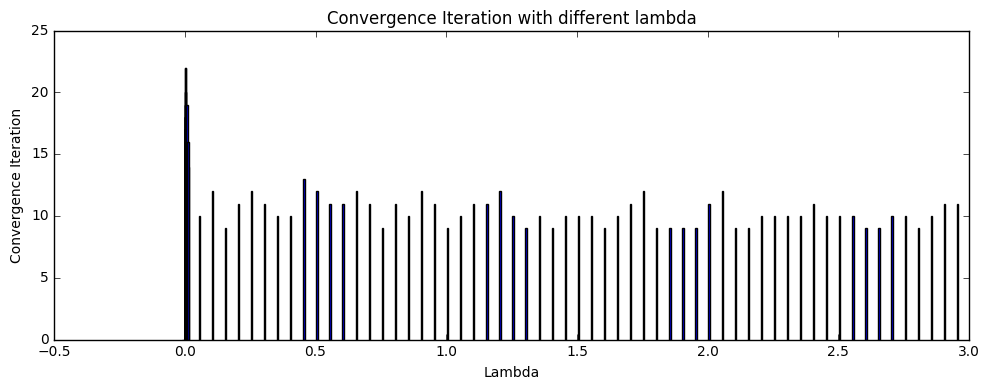
\includegraphics[width=16cm]{../model/lambda_iter.png}
\end{center}
\caption{Convergence Iteration with a set of $\lambda$ on a9a with IRLS(L2).}\label{lambda_iter}
\end{figure}
Figure \ref{lambda_iter} shows the Convergence Iteration of a set of $\lambda$.  So the We can see that, when $\lambda \approx 0$, the convergence iteration is more than 20 times, when $\lambda \ge 0.1$, the convergence iteration is about 10 times, it shows that the L2 normalized IRLS has a fast convergence speed than IRLS. 


\begin{figure}[!htbp]
\begin{center}
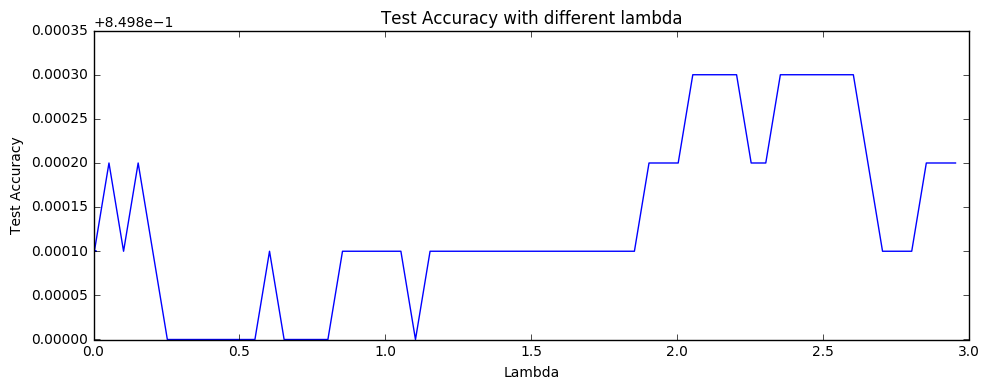
\includegraphics[width=16cm]{../model/lambda_acc.png}
\end{center}
\caption{Test Accuracy with a set of $\lambda$ on a9a with IRLS(L2).}\label{lambda_acc}
\end{figure}

Figure \ref{lambda_acc} shows the Test Accuracy of a set of $\lambda$.  So the We can see that, when $\lambda \approx 0$, the convergence iteration is more than 20 times, when $\lambda \ge 0.1$, the convergence iteration is about 10 times, it shows that the L2 normalized IRLS has a fast convergence speed than IRLS. 

\begin{figure}[!htbp]
\begin{center}
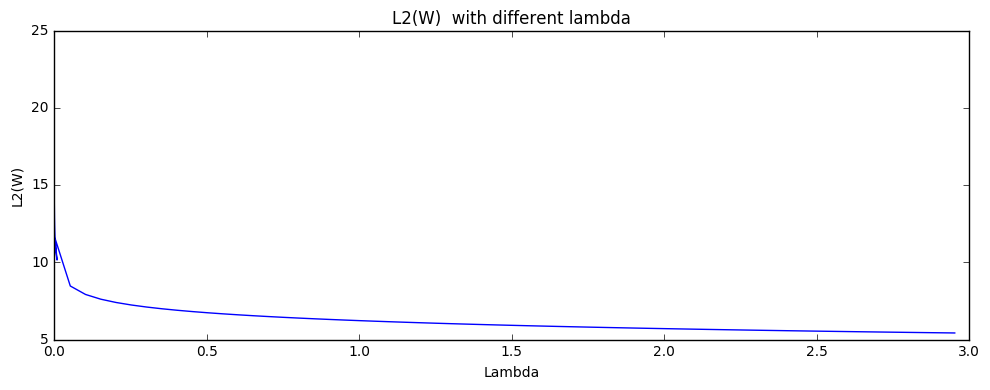
\includegraphics[width=16cm]{../model/lambda_l2norm.png}
\end{center}
\caption{The L2 norm value of $W$ with a set of $\lambda$ on a9a.}\label{lambda_l2norm}
\end{figure}

Figure \ref{lambda_l2norm} shows the L2 norm value of $W$ with a set of $\lambda$.  The $W$ is decreased when $\lambda$ is larger. 


%[!htbp]
\begin{figure}[!htbp]
\begin{center}
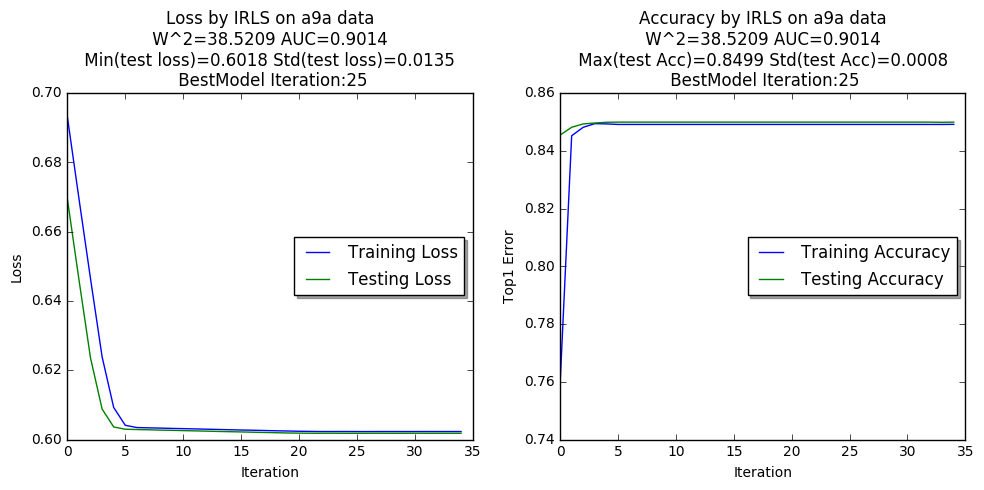
\includegraphics[width=16cm]{../model/IRLS.png}
\end{center}
\caption{Training performance with IRLS on "UCI a9a" dataset.}\label{IRLS}
\end{figure}
Figure \ref{IRLS} shows the loss and the accuracy curve by IRLS with the earlystoping on "UCI a9a" dataset.  The best model (validation loss is minimum ) is at iteration 25, and the loss ($J(W)$) is 0.6018, $\Vert W \Vert_2^2$ is 38.5209, the best test accuracy is 0.8499, the AUC is 0.9014. 

\begin{figure}[!htbp]
\begin{center}
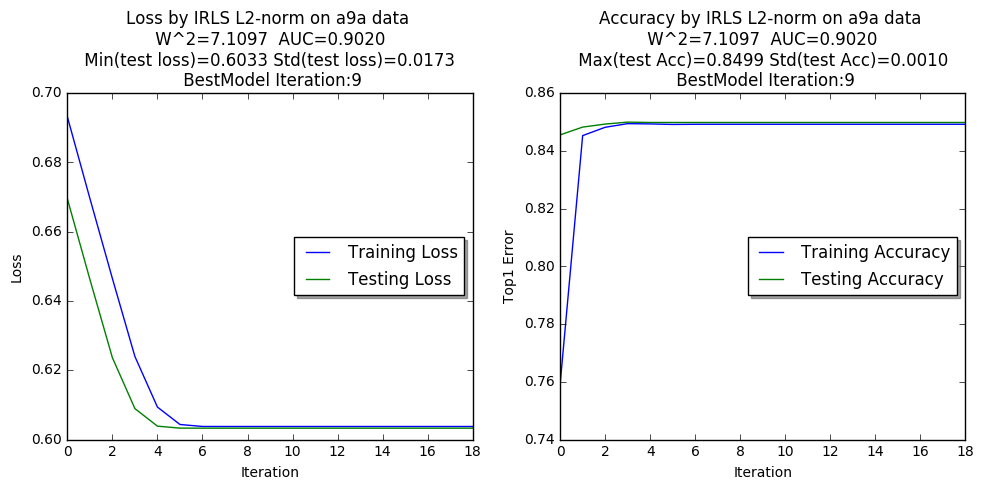
\includegraphics[width=16cm]{../model/IRLS_L2_w_0.3.png}
\end{center}
\caption{Training performance with L2 normalized IRLS on "UCI a9a" dataset.}\label{IRLS_L2}
\end{figure}

Figure \ref{IRLS_L2} shows the loss and the accuracy curve by L2 normalized IRLS with the earlystoping on "UCI a9a" dataset.  The best model (validation loss is minimum ) is at iteration 9, and the loss ($J(W)$) is 0.6033, $\Vert W \Vert_2^2$ is 7.1097, the best test accuracy is 0.8499, the AUC is 0.9020. 

\bibliographystyle{plain}
%\bibliography{bibliography.bib}
\end{document}